\chapter{Lösungsansatz}
\label{ch:loesungsansatz}

\section{Selbstlernende KI mithilfe von Trainingsdaten}
\label{sec:selbstlernende-ki-trainingsdaten}

Zunächst haben wir uns die Frage gestellt, ob eine \ac{KI} mithilfe von Trainingsdaten lernen soll.
Dieser Ansatz bringt jedoch das Problem mit sich, gute Trainingsdatensätze besitzen zu müssen.
Bei einer maximalen Anzahl von sechs Spielern im Spiel \texttt{spe\_ed} und 5 unterschiedlichen möglichen Aktionen gibt
es sehr viele Möglichkeiten, wie ein Spiel verlaufen kann.
Dabei entsteht das Problem zu beurteilen, welche Spielsituationen und welche Spielverläufe als Trainingsdaten gut
geeignet sind, sodass die gesamte Komplexität des Spiels in unseren Trainingsdaten abgebildet wird.
Aufgrund dessen haben wir uns dafür entschieden, zunächst Lösungsansätze ohne eine selbstlernende \ac{KI}
auszuprobieren.
Diese Strategie hatte für uns den Vorteil, mithilfe einfacherer Lösungsansätze die Komplexität und auftretenden Probleme
im Spielverlauf besser kennen zu lernen. \todo{weitere technische Begründung hinzufügen}

\section{Lösungsansätze ohne selbstlernende KIs}
\label{sec:loesungsansatz-ohne-selbstlernende-kis}

Bei dem Ansatz, Strategien fest in Code zu implementieren, hatten wir mehrere unterschiedliche Ideen,
die nachfolgend beschrieben werden.
Ziel war es hierbei, Teilprobleme zu erkennen und zu lösen, mit der Intuition diese unterschiedlichen \ac{KI}s
kombinieren zu können.

\subsection{RandomAI}
\label{subsec:random-ai}

Die \Code{RandomAI} ist unsere erste lauffähige KI gewesen und unser Maß für die einfachste \ac{KI}.
Diese stellt zwar keinen wirklichen Lösungsansatz dar, diente jedoch als Einstieg und um erste Probleme zu erkennen.
Durch die \Code{RandomAI} ist uns das grundlegende Problem aufgefallen, dass sich die \ac{KI} selber tötet.
Folglich wird die Minimal- und Maximalgeschwindigkeit überschritten, das Spielfeld verlassen oder in vorhandene Spuren
gefahren, mit denen eine Kollision vermeidbar gewesen wäre.

\subsection{NotKillingItselfAI}
\label{subsec:notkillingitself-ai}

Aufgrund des beschriebenen Problemes der \Code{RandomAI} haben wir uns dafür entschieden, die \Code{NotKillingItselfAI}
zu implementieren.
Die \ac{KI} soll aus allen Aktionen eine zufällige Aktion auswählt, die sie nicht direkt verlieren lässt.
Dazu wird für jede mögliche Aktion die Spur berechnet, die entstehen würde und auf Kollisionen überprüft.
Aktionen die eine Kollision hervorrufen werden nicht ausgeführt.
Hierbei bleiben mögliche Aktionen der Gegenspieler zunächst unberücksichtigt. \\

Durch die Implementierung der \Code{NotKillingItselfAI} fiel auf, dass die \ac{KI} sich zwar nicht mehr im unmittelbar
folgenden Zug tötete, jedoch häufig in Sackgassen läuft.
Dieses Problem wird in der \Abbildung{fig:Sackgassen_Problem} verdeutlicht.

\begin{figure}[htb]
    \centering
    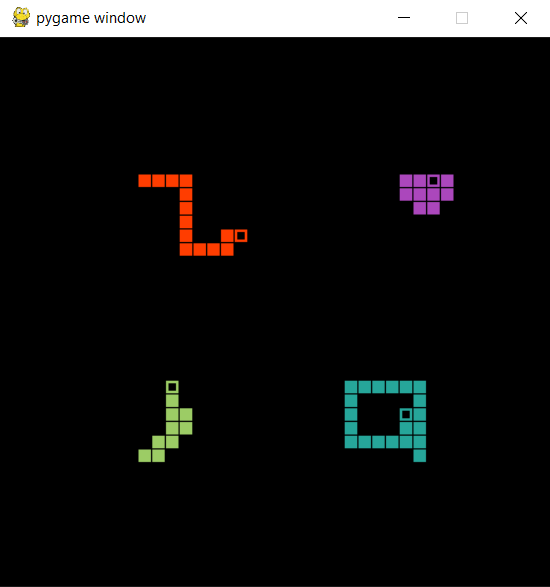
\includegraphics[width=0.6\textwidth]{Bilder/Sackgassen_Problem.png}
    \caption{\Code{NotKillingItselfAI} unten rechts in einer Sackgasse}
    \label{fig:Sackgassen_Problem}
\end{figure}

\subsection{PathfindingAI}
\label{subsec:pathfinding-ai}

Folglich der \Code{NotKillingItselfAI} haben wir einen Lösungsansatz gesucht, welcher das Betreten von Sackgassen
verhindert.
Genutzt wurde die Basis der \Code{NotKillingItselfAI}, sodass nur zwischen überlebenden Aktionen gewählt wird.
Um die Aktionen zu finden, die nicht in eine Sackgasse läuft, haben wir uns für einen Lösungsansatz zum Finden von
Pfaden entschieden.
Dazu wird eine konfigurierbare Anzahl zufälliger Koordinaten generiert, auf denen sich bisher kein Spieler befindet.
Anschließend wird für jede Aktion geprüft, zu wie vielen der Koordinaten, nach der Ausführung der Aktion noch ein
möglicher Pfad existiert. \todo{In einem Bild verdeutlichen warum das ein Bewertungskriterium darstellt}
Die Aktion, die die höchste Anzahl Koordinaten erreichen kann, führt mit höchster Wahrscheinlichkeit
nicht in eine Sackgasse und wird ausgewählt. \\

Bei diesem Lösungsansatz arbeiten wir lediglich mit der Wahrscheinlichkeit, dass wir nicht in eine Sackgasse laufen.
Dies liegt dem Problem zugrunde, dass wir die Implementierung eines Algorithmus zum tatsächtichen Erkennen von
Sackgassen oder abgesperrten Gebieten als schwieriger erachteten. \\

Wir haben die Python-Bibliothek \Code{pathfinding} verwendet, die bereits unterschiedliche Algorithmen zum Finden von
Pfaden in einem Graphen bietet.
Die Entscheidung welcher Algorithmus zum Finden eines Pfades verwendet wird hat eine große Auswirkung auf die
Performance der \Code{PathfindingAI}.
Der Algorithmus stellt den Flaschenhals dar, da dieser je nach Konfiguration mehrere hundert bis tausend mal pro
Zug ausgeführt werden muss.
Wir haben die unterschiedlichen Algorithmen hinsichtlich ihrer Ausführungsdauer verglichen und uns folglich für die
Verwendung vom Best-First-Algorithmus entschieden.
Bei dem Vergleich wurde in 50 unterschiedlichen Spielsituationen jeweils 200 Pfade für jede mögliche Aktion gesucht, um
den schnellsten Algorithmus zu finden.
Die durchschnittlichen Ausführungzeiten auf unserem Testrechner können der
\Tabelle{tab:ausfuehrungsdauer-pfadalgorithmen} entnommen werden.

\begin{table}[htb]
    \centering
    \begin{tabular}{|l|l|}
        \hline
            \textbf{Algorithmus} & {\textbf{Durchschnittliche Ausführungsdauer in Sekunden}} \\ \hline
            BestFirst 		    & 0.740099930763244 \\ \hline
            BiAStarFinder 		& 0.994705820083618 \\ \hline
            AStarFinder 		& 1.257498860359192 \\ \hline
            BreadthFirstFinder  & 1.376600646972656 \\ \hline
            DijkstraFinder		& 2.440193486213684 \\ \hline
    \end{tabular}
    \caption{Ausführungsdauer unterschiedlicher Algorithmen zum Finden von Pfaden}
    \label{tab:ausfuehrungsdauer-pfadalgorithmen}
\end{table}

\subsection{SearchTreeAI}
\label{subsec:searchtree-ai}

Bei der \Code{PathfindingAI}, als auch der \Code{NotKillingItselfAI} gibt es weiterhin ein bestehendes
Problem.
Die \ac{KI} beachtet die möglichen Aktionen der Gegenspieler nicht.
Ziel der \Code{SearchTreeAI} ist es, dass die die \Code{NotKillingItselfAI}, falls möglich, auch nur Aktionen berechnet,
bei denen bereits alle möglichen gegnerischen Aktionen und dessen Auswirkungen berücksichtigt werden. \\

Unser Lösungsansatz für dieses Problem ist es, mithilfe eines Suchbaums alle möglichen gegnerischen
Aktions-Kombinationen zu prüfen und einen Teilbaum zu finden, bei dem vorausgesagt werden kann, dass
der eigene Spieler unabhängig der ausgewählten Aktion von allen anderen Spielern nicht im nächsten Zug stirbt.
Der Vorteil eines Suchbaums ist es, dass wir diesem eine
beliebige Tiefe mitgeben können, um entsprechend der Tiefe viele zukünftige Züge vor zu berechnen.
\todo{Besser ausformulieren, Problem der Komplexität benennen und Beispielskizze}

\section{Vorgehen zur Auswahl der besten Strategie}
\label{sec:vorgehen-strategieauswahl}
